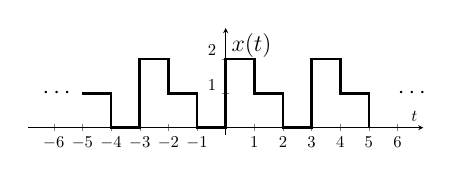
\begin{tikzpicture}[scale=0.6]
    \begin{axis}[
        x=.05\textwidth,y=0.06\textwidth,
    	axis y line=center,
    	axis x line=middle,
    	xlabel=$t$,ylabel={\Large $x(t)$},
    	xmin=-6.9,xmax=6.9,
    	ymin=-0.2,ymax=2.9,
    	xtick={-6,...,6},
    	xticklabel style = {xshift=0},
    	yticklabel style = {yshift=5}
	] 
	\addplot[
    	black,
    	ultra thick
    	] coordinates {
	(-5,1) (-4,1) (-4,0) (-3,0) (-3,2) (-2,2) (-2,1) (-1,1) (-1,0) (0,0) (0,2) (1,2) (1,1) (2,1) (2,0) (3,0) (3,2) (4,2) (4,1) (5,1) (5,0)
	} ;
	\node at (axis cs:6.5,1) {\Large $\cdots$} ;
	\node at (axis cs:-5.9,1) {\Large $\cdots$} ;
    \end{axis}
\end{tikzpicture}